\documentclass[10pt,a4paper]{article}
\usepackage{amsmath}
\usepackage{amssymb}
\usepackage{graphicx}
\usepackage{color}
\usepackage{fancyhdr}
\usepackage{fancyvrb}
\usepackage[margin=3.5cm]{geometry}
\usepackage{framed}
\usepackage{enumerate}
\usepackage{textcomp}
\def\ket#1{\left|#1\right\rangle}
\def\bra#1{\left\langle#1\right|}
\def\braket#1{\left\langle#1\right\rangle}

\FrameSep 8pt
\setlength{\topsep}{1pt}

\definecolor{linkcol}{rgb}{0.0, 0.0, 0.5}
\usepackage[colorlinks=true,urlcolor=linkcol,citecolor=black,linkcolor=linkcol]{hyperref}

\renewcommand\thesection{10.\arabic{section}}
\renewcommand\thesubsection{\thesection.\arabic{subsection}}

\fancyhf{}
\lhead{\tiny Y.~D.~Chong (2016)}
\rhead{\scriptsize MH2801: Complex Methods for the Sciences}
\lfoot{}
\rfoot{\thepage}
\pagestyle{fancy}

\makeatletter
\def\PY@reset{\let\PY@it=\relax \let\PY@bf=\relax%
    \let\PY@ul=\relax \let\PY@tc=\relax%
    \let\PY@bc=\relax \let\PY@ff=\relax}
\def\PY@tok#1{\csname PY@tok@#1\endcsname}
\def\PY@toks#1+{\ifx\relax#1\empty\else%
    \PY@tok{#1}\expandafter\PY@toks\fi}
\def\PY@do#1{\PY@bc{\PY@tc{\PY@ul
\def\PYZdl{\char`\$}
\def\PYZhy{\char`\-}
\def\PYZsq{\char`\'}
\def\PYZdq{\char`\"}
\def\PYZti{\char`\~}

\begin{document}
\setcounter{page}{81}
\noindent
\underline{\textbf{\LARGE 10. Green's functions}}
\vskip 0.1in

A \textbf{Green's function} is a solution to an inhomogenous
differential equation with a ``driving term'' given by a delta
function. It is used as a convenient method for solving more
complicated inhomogenous differential equations. In physics, Green's
functions methods are used to describe a wide variety of phenomena,
ranging from the motion of complex mechanical oscillators to the
emission of sound waves from loudspeakers.

\section{The driven harmonic oscillator}
\label{driven-oscillator}

As an introduction to the Green's function technique, we study the
\textbf{driven harmonic oscillator}, which is a damped harmonic
oscillator subjected to an arbitrary driving force. Its equation of
motion is
\begin{equation}
  \left[\frac{d^2}{dt^2} + 2 \gamma \frac{d}{dt} + \omega_0^2\right] x(t) = \frac{f(t)}{m}.
  \label{driven_eq}
\end{equation}
The left-hand side is the same as in the damped harmonic oscillator
equation (see Chapter 4), where $m$ is the mass of the particle,
$\gamma$ is the damping coefficient, and $\omega_0$ is the natural
frequency of the oscillator. On the right-hand side, we introduce a
time-dependent driving force $f(t)$ (which acts alongside the
pre-existing spring and damping forces). Given an arbitrarily
complicated $f(t)$, our goal is to determine $x(t)$.

\subsection{Green's function for the driven harmonic oscillator}
\label{greens-function-for-the-driven-harmonic-oscillator}

Prior to solving the driven harmonic oscillator problem for a general
driving force $f(t)$, let us first consider the following equation:
\begin{equation}
  \left[\frac{\partial^2}{\partial t^2}
    + 2 \gamma \frac{\partial}{\partial t}
    + \omega_0^2\right] G(t, t') = \delta(t-t').
  \label{osc_green}
\end{equation}
This is called the \textbf{Green's function equation}. The function
$G(t,t')$, which depends on the two variables $t$ and $t'$, is called
the \textbf{Green's function}. Note that the differential operator on
the left-hand side involves only derivatives in $t$.

Comparing Eq.~(\ref{osc_green}) to Eq.~(\ref{driven_eq}), we see that
$G(t,t')$ describes the motion of a damped harmonic oscillator that is
subjected to a particular choice of driving force---an infinitesimally
sharp pulse centered at $t = t'$. This pulse is described by a delta
function (see Section 9.4):
\begin{equation}
  f(t) = m\,\delta(t-t').
\end{equation}

Why do we care about the Green's function? The reason is that as soon
as $G(t,t')$ is known, we can easily produce a specific solution to
the driven harmonic oscillator equation for \emph{any} given driving
force $f(t)$. That solution has the following form:
\begin{equation}
  x(t) = \int^\infty_{-\infty} dt' \; G(t,t') \; \frac{f(t')}{m}.
  \label{greenx}
\end{equation}
To show mathematically that this is indeed a solution, plug
Eq.~(\ref{greenx}) into Eq.~(\ref{driven_eq}):
\begin{align}
  \begin{aligned}
    \left[\frac{d^2}{dt^2} + 2 \gamma \frac{d}{dt} + \omega_0^2\right]\, x(t)
    &= \int^\infty_{-\infty} dt' \; \left[\frac{\partial^2}{\partial t^2}
      + 2 \gamma \frac{\partial}{\partial t} + \omega_0^2\right] G(t,t')
    \frac{f(t')}{m} \\ &= \int^\infty_{-\infty} dt' \; \delta(t-t')\,
    \frac{f(t')}{m} \\ &= \frac{f(t)}{m}.
  \end{aligned}
\end{align}
(Note that we can move the differential operator inside the integral
over $t'$ because $t$ and $t'$ are independent variables.) We have
thus shown that the above expression for $x(t)$ satisfies the driven
oscillator equation for driving force $f(t)$.

The Green's function concept is based on the principle of
superposition of waves and oscillations. The motion of the oscillator
is induced by the driving force, but the value of $x(t)$ at time $t$
does not just depend on the instantaneous value of $f(t)$ at time $t$,
but rather on the values of $f(t')$ over all times $t' < t$. (Indeed,
the oscillations will continue even after the driving force is turned
off.)  The key idea is that any function $f(t)$ can be decomposed into
a superposition of delta functions. Since the response of the
oscillator to a delta function force is given by the Green's function,
the solution $x(t)$ is given by a superposition of Green's functions.

\subsection{Finding the Green's function}
\label{finding-the-greens-function}

To solve the Green's function equation, we use the Fourier
transform. Let us suppose for now that the Fourier transform of
$G(t,t')$ with respect to $t$ is convergent (we'll examine this
assumption in detail later, in
\hyperref[causality]{Section~\ref{causality}}). We will also assume
that the oscillator is not critically damped, i.e.~$\omega_0 \ne
\gamma$.

The Fourier-transformed Green's function is called the
\textbf{frequency-domain Green's function}:
\begin{equation}
  G(\omega, t') = \int_{-\infty}^\infty dt \; e^{i\omega t}\, G(t,t').
\end{equation}
Note that we have used the usual sign convention for time-domain
Fourier transforms (see Section~9.2.3).

Next, we Fourier transform both sides of the Green's function equation
(\ref{osc_green}), and make use of how derivatives behave under
Fourier transformation. The result is
\begin{equation}
  \left[- \omega^2 - 2i \gamma\omega + \omega_0^2\right] G(\omega,t')
  = \int_{-\infty}^\infty dt \; e^{i\omega t}\, \delta(t-t') = e^{i\omega t'}.
\end{equation}
The differential equation for $G(t,t')$ has thus been converted into
an \emph{algebraic} equation for $G(\omega,t')$. The latter is easily
solved:
\begin{equation}
  G(\omega, t') = - \frac{e^{i\omega t'}}{\omega^2 + 2i\gamma\omega - \omega_0^2}.
\end{equation}
Finally, we retrieve the time-domain solution by using the inverse
Fourier transform:
\begin{align}
  G(t,t') &= \int_{-\infty}^\infty \frac{d\omega}{2\pi} \,
  e^{-i\omega t} G(\omega, t')  \\&= - \int_{-\infty}^\infty \frac{d\omega}{2\pi}
  \, \frac{e^{-i\omega (t-t')}}{\omega^2 + 2i\gamma\omega - \omega_0^2}.
\end{align}
The denominator of the integral is a quadratic expression, so this can
be re-written as:
\begin{equation}
  G(t,t') = - \int_{-\infty}^\infty \frac{d\omega}{2\pi} \,
  \frac{e^{-i\omega (t-t')}}{(\omega - \omega_+)(\omega - \omega_-)}
  \quad\mathrm{where}\;\; \omega_{\pm} = -i\gamma \pm
  \sqrt{\omega_0^2-\gamma^2}.
\end{equation}
This can be evaluated by contour integration. The integrand has two
poles, both lying in the negative complex plane (note: these are
precisely the complex frequencies of the damped harmonic oscillator
discussed in Chapter 4). For $t < t'$, Jordan's lemma requires us to
close the contour in the upper half-plane; this encloses neither pole,
so the integral is zero. For $t > t'$, we must close the contour in
the lower half-plane, enclosing both poles. The result is
\begin{align}
  G(t,t') &= i \Theta(t-t') \,
  \left[ \frac{e^{-i\omega_+ (t-t')}}{\omega_+ - \omega_-}
    + \frac{e^{-i\omega_- (t-t')}}{\omega_- - \omega_+}\right] \\
  &= \Theta(t-t') \;e^{-\gamma(t-t')} \; \times
  \left\{\begin{array}{ll} \frac{1}{\sqrt{\omega_0^2-\gamma^2}}\,
  \sin\left[\sqrt{\omega_0^2-\gamma^2} (t-t')\right],
  & \gamma < \omega_0, \\
  \frac{1}{\sqrt{\gamma^2-\omega_0^2}}\,
  \sinh\left[\sqrt{\gamma^2-\omega_0^2} (t-t')\right],
  & \gamma > \omega_0.\end{array}\right.
\end{align}
Here, $\Theta(t-t')$ refers to the step function
\begin{equation}
  \Theta(\tau) = \left\{\begin{array}{ll} 1, &\;\;\;\textrm{for}
  \; \tau \ge 0\\ 0,&\;\;\; \textrm{otherwise.}\end{array}\right.
\end{equation}
This result is plotted in the figure below, in both the under-damped
and over-damped regimes. The solution for the critically-damped case,
$\gamma = \omega_0$, is left as an \hyperref[exercises]{exercise}.

\begin{figure}[h]
  \centering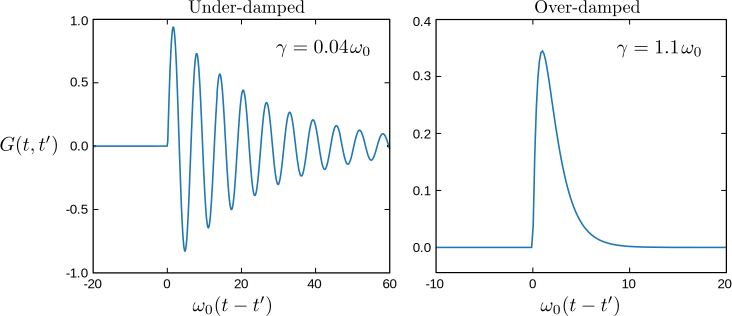
\includegraphics[width=0.7\textwidth]{oscillator_greenfun}
\end{figure}
    
\subsection{Features of the Green's function}
\label{features}

As previously noted, the time-domain Green's function has a physical
meaning: it represents the motion of the oscillator in response to a
force ``pulse'', $f(t) = m\, \delta(t-t')$. The basic features of the
results obtained \hyperref[finding-the-greens-function]{in the
  previous section} match our intuition of what this motion should
look like.

The first thing to notice is that the Green's function depends on $t$
and $t'$ only in the combination $t-t'$. In physical terms, it is easy
to see why: the response of the oscillator to an infintesimally sharp
force pulse should only depend on the time elapsed since the pulse. To
take advantage of this property, we could re-define the
frequency-domain Green's function as
\begin{equation}
  G(\omega) = \int_{-\infty}^\infty dt \; e^{i\omega (t-t')}\, G(t-t'),
\end{equation}
which then obeys
\begin{equation}
  \left[- \omega^2 - 2i \gamma\omega + \omega_0^2\right] G(\omega) = 1.
\end{equation}
This is a little nicer to work with, because there isn't an extraneous
$t'$ variable in the definition.

The next thing to notice is how the Green's function behaves just
before and after the pulse. Its value is zero for $t - t' < 0$ (i.e.,
prior to the application of the pulse). This feature is referred to as
``causality'', and we will discuss it in greater detail
\hyperref[causality]{in Section~\ref{causality}}. Moreover, there is
no discontinuity in $x(t)$ at $t - t' = 0$, which means that the force
pulse does not cause the oscillator to ``teleport'' instantaneously to
a different position. Rather, it produces a discontinuity in the
oscillator's \emph{velocity}.

To see this explicitly, let us integrate the Green's function equation
(\ref{osc_green}) over an infinitesimal interval of time surrounding
$t'$:
\begin{align}
  \begin{aligned}
    \lim_{\epsilon \rightarrow 0} \int_{t'-\epsilon}^{t'+\epsilon} dt
    \left[\frac{\partial^2}{\partial t^2} + 2\gamma\frac{\partial}{\partial t}
      + \omega_0^2\right] G(t,t') &= \lim_{\epsilon \rightarrow 0}
    \int_{t'-\epsilon}^{t'+\epsilon} dt \; \delta(t-t') \\
    = \lim_{\epsilon \rightarrow 0} \left\{ \left.\frac{\partial G(t,t')}{\partial t}
    \right|_{t = t' +\epsilon}
    - \left.\frac{\partial G(t,t')}{\partial t}\right|_{t = t' - \epsilon}\right\}
    &= 1
  \end{aligned}
\end{align}
On the last line, the expression on the left-hand side represents the
difference between the oscillator velocity just after the pulse, and
the velocity just before the pulse. Evidently, the force pulse imparts
one unit of velocity at $t=t'$. If you look at the solutions obtained
\hyperref[finding-the-greens-function]{in the previous section}, you
can verify that indeed $\partial G/\partial t = 0$ immediately before
the pulse, and $\partial G/\partial t = 1$ immediately after the
pulse.

For $t - t' > 0$, the applied force goes back to zero, and the system
behaves like the undriven harmonic oscillator. If the oscillator is
under-damped ($\gamma < \omega_0$), it undergoes oscillation around
the origin, which decays exponentially back to the origin as the
energy imparted by the pulse is damped away. If the oscillator is
over-damped ($\gamma > \omega_0$), the oscillator moves for a
distance, then decays exponentially back to the origin without
oscillating.

\subsection{Causality}\label{causality}

We have noted that the motion $x(t)$ ought to depend on the driving
force $f(t')$ at all past times $t' < t$, but should \emph{not} depend
on the force at future times. Because of the relation
\begin{equation}
  x(t) = \int_{-\infty}^\infty dt'\; G(t,t')\, \frac{f(t')}{m},
\end{equation}
this means that the Green's function ought to satisfy
\begin{equation}
  G(t,t') = 0 \;\; \mathrm{for}\;\; t -t' < 0.
\end{equation}
This condition is referred to as \textbf{causality}, because it is
equivalent to saying that \emph{cause} must precede \emph{effect}. A
Green's function that satisfies it is called a \textbf{causal Green's
  function}. The specific solution for $G(t,t')$ which we
\hyperref[finding-the-greens-function]{derived in
  Section~\ref{finding-the-greens-function}} is a causal Green's
function.

The time-domain Green's function satisfies a second-order differential
equation, so it has a family of solutions; the general solution
contains two free parameters. Not all solutions for the time-domain
Green's function are causal. We need to ask ourselves whether the
specific solution we found in the previous section is the \emph{only}
possible causal solution. It turns out that the answer is yes, and
there are a couple of ways to see why.

The first approach is to observe that for $t > t'$, the Green's
function satisfies the differential equation for the \emph{undriven}
harmonic oscillator.  But as we noted in
\hyperref[features]{Section~\ref{features}}, the Green's function must
also obey two conditions at $t = t' + 0^+$: (i) $G = 0$, and (ii)
$\partial G / \partial t = 1$. These act as two boundary conditions
for the undriven harmonic oscillator equation over the range $t > t'$.
Hence, the solution for $G(t,t')$ in this range is completely
specified.

The other way to see that the causal Green's function is unique is to
imagine adding to our specific solution any solution $x_1(t)$ for the
undriven harmonic oscillator. It is easy to verify that the new form
of $G(t,t')$ is still a solution to the differential equation for the
Green's function. As we saw during our study of the damped harmonic
oscillator (Chapter 4), the general solution for $x_1(t)$ contains two
free parameters. The general solution is always infinite for $t
\rightarrow -\infty$, with one exception: the ``trivial'' solution
$x_1(t) = 0$. The trivial solution is a \emph{specific}
solution. Thus, the causality requirement is equivalent to setting
\emph{two} boundary conditions, so the causal Green's function that we
have found is the only possible one.

Moreover, if we add a non-trivial undriven oscillator solution
$x_1(t)$ to the Green's function, the Green's function would no longer
have a convergent Fourier transform---it wouldn't be square-integrable
due to blowing up in the $t \rightarrow -\infty$ limit. Hence,
requiring the time-domain Green's function to obey causality is
equivalent to requiring the frequency-domain Green's function to be
well-defined.

\section{Space-time Green's functions}
\label{space-time-greens-functions}

We can also use the Green's function method to study the wave
equation, in order to describe the emission (and absorption) of
waves. For simplicity, we restrict our discussion to waves propagating
through a uniform medium (i.e., a medium that is featureless through
all of space and time). Let us also assume that there is a single
space dimension, given by coordinate $x$. (The generalization of the
following discussion to the case of multiple spatial dimensions will
be pretty straightforward.)

As we saw in Chapter 5, it is convenient to describe a wave using a
complex wavefunction $\psi(x,t)$, which obeys the wave equation
\begin{equation}
  \left[\frac{\partial^2}{\partial x^2} - \left(\frac{1}{c}\right)^2 \frac{\partial^2}{\partial t^2} \right] \psi(x,t) = 0.
\end{equation}
Here, $c$ is the speed of wave propagation. Henceforth, to simplify
the equations, we will set $c = 1$. (You can go back to the previous
case by replacing all instances of $t$ with $c t$, and $\omega$ with
$\omega/c$, in the formulas that we will derive.)

The wave equation describes how waves propagate \emph{after} they have
already been created. To describe how the waves are generated in the
first place, we must modify the wave equation by introducing a term on
the right-hand side, called a \textbf{source}:
\begin{equation}
  \left[\frac{\partial^2}{\partial x^2} - \frac{\partial^2}{\partial t^2} \right] \psi(x,t)\, = f(x,t).
\end{equation}
The source term turns the wave equation into an inhomogenous partial
differential equation. It plays a role very similar to the driving
force in the driven harmonic oscillator problem from
\hyperref[driven-oscillator]{Section~\ref{driven-oscillator}}.  In
acoustics, for example, such a source term can describe the motion of
a loudspeaker's membrane, and $\psi(x,t)$ describes the waves that are
emitted by the loudspeaker.

\subsection{Time-domain Green's function}
\label{time-domain-greens-function}

The wave equation's \textbf{time-domain Green's function} is defined
by setting the source term to delta functions in both space and time:
\begin{equation}
  \left[\frac{\partial^2}{\partial x^2}
    - \frac{\partial^2}{\partial t^2} \right] G(x,x';t-t')
  = \delta(x-x')\, \delta(t-t').
\end{equation}
As can be seen, $G$ is a function of two spatial variables, $x$ and
$x'$, as well as two temporal variables $t$ and $t'$. It corresponds
to the wave generated by a pulse
\begin{equation}
f(x,t) = \delta(x-x')\,\delta(t-t').
\end{equation}
The differential operator in the Green's function equation only
involves $x$ and $t$, so we can regard $x'$ and $t'$ as parameters
specifying where the pulse is localized in space and time. This
Green's function ought to depend on the time variables only in the
combination $t-t'$, similar to our previous discussion of the Green's
function for the driven harmonic oscillator
(\hyperref[driven-oscillator]{Section~\ref{driven-oscillator}}); to
emphasize this, we have written it as $G(x,x';t-t')$.

Just as for the harmonic oscillator, we can use the Green's function to
construct a solution for the driven wave equation with an arbitrary
source:
\begin{equation}
\psi(x,t) = \int dx' \,\int_{-\infty}^\infty dt'\; G(x,x';t-t') \, f(x', t').
\end{equation}
This difference from the harmonic oscillator problem is that the
Green's function and the source now depend on space as well as time,
so we also need to integrate over space in order to obtain
$\psi(x,t)$. The Green's function thus contains information about how
the influence of the source at one point in space and time
\emph{propagates} to other points in both space and time.

\subsection{Frequency-domain Green's function for waves}
\label{frequency-domain}

The wave equation's \textbf{frequency-domain Green's function} is
obtained by Fourier transforming the time-domain Green's function in
the $t-t'$ coordinate:
\begin{equation}
  G(x,x';\omega) = \int_{-\infty}^\infty d\tau\; e^{i\omega \tau}\, G(x,x'; \tau).
\end{equation}
It obeys the differential equation
\begin{equation}
  \left[\frac{\partial^2}{\partial x^2} + \omega^2 \right]
  G(x,x';\omega) = \delta(x-x').
\end{equation}
Just as we can write the time-domain solution to the wave equation in
terms of the time-domain Green's function, we can do the same for the
frequency-domain solution:
\begin{equation}
  \Psi(x,\omega) = \int dx' \; G(x,x';\omega) \, F(x', \omega),
\end{equation}
where
\begin{equation}
  \Psi(x,\omega) = \int_{-\infty}^\infty dt \; e^{i\omega t} \, \psi(x,t),
  \quad F(x,\omega) = \int_{-\infty}^\infty dt \; e^{i\omega t} \, f(x,t).
\end{equation}
Note that there is no integral over frequencies: the $\omega$
component of the solution involves only the $\omega$ components of the
Green's function and the $-\omega$ components of the source
contribute, without any contribution from other frequencies.

\subsection{Outgoing boundary conditions}
\label{outgoing}

In order to find the time-domain Green's function, it is simplest to
solve for the frequency-domain Green's function first (we pursued a
similar strategy when dealing with the
\hyperref[driven-oscillator]{harmonic oscillator Green's function}).

Before looking for a solution, we need to specify the boundary
conditions. That, however, depends on the situation we are interested
in. One common setup is a enclosed cavity, where the waves propagate
inside a finite domain, say $x \in (x_a,x_b)$. For such situations, we
usually impose \textbf{Dirichlet boundary conditions}, which state
that $G(x,x';\omega) = 0$ at the edges of the domain. The
frequency-domain Green's function can then be solved by decomposing it
into a series of basis functions defined within the finite domain,
analogous to the Fourier series.

We will instead focus on a more interesting situation, which occurs
when the space coordinate is unbounded, and runs over the entire space
$x \in (-\infty, \infty)$. This describes, for example, a loudspeaker
that emits sound into empty space, or an antenna that radiates
electromagnetic waves into empty space. The emitted waves should
propagate outward from the source, and the boundary conditions
describing this condition are called \textbf{outgoing boundary
  conditions}. In 1D, this means that the Green's function should
correspond to a left-moving wave for all $x$ to the left of the
source, and to a right-moving wave for all $x$ to the right of the
source.

We can guess the form of the Green's function which obeys such
boundary conditions:
\begin{equation}
  G(x,x';\omega) = \left\{\begin{array}{ll}A \, e^{-i\omega (x-x')}, & x \le x',
  \\ B \, e^{i\omega (x-x')}, & x \ge x'\end{array}\right.
  \quad \mathrm{for}\;\mathrm{some}\;\; A, B \in \mathbb{C}.
\end{equation}
It is straightforward to verify that this formula for $G(x,x',\omega)$
satisfies the wave equation in both the regions $x < x'$ and $x > x'$,
and that it satisfies outgoing boundary conditions. We simply have to
determine the $A$ and $B$ coefficients. To do this, first note that
$G(x,x')$ should be continuous at $x = x'$, so $A = B$.

Secondly, integrating the Green's function equation across $x'$ gives
\begin{align}
  \begin{aligned}
  \lim_{\epsilon \rightarrow 0} \int_{x'-\epsilon}^{x'+\epsilon}
  \left[\frac{\partial^2}{\partial x^2} + \omega^2\right]G(x-x')
  &= \lim_{\epsilon \rightarrow 0} \int_{x'-\epsilon}^{x'+\epsilon} \delta(x-x') \\
  = \lim_{\epsilon \rightarrow 0} \left\{ \left.\frac{\partial G}{dx} (x,x')
  \right|_{x = x'+\epsilon} - \left.\frac{\partial G}{\partial x} (x,x')
  \right|_{x = x'-\epsilon}\right\} &= i\omega (B + A) = 1.
  \end{aligned}
\end{align}
Combining these two equations gives $A = B = 1/2i\omega$. Hence, the
Green's function for outgoing boundary conditions is
\begin{equation}
G(x,x';\omega) = \frac{e^{i\omega |x-x'|}}{2i\omega}.
\end{equation}

\subsection{Causality and the time-domain Green's function}
\label{causality-and-the-time-domain-greens-function}

The outgoing frequency-domain Green's function derived in the previous
section can be converted to a time-domain Green's function by the
usual inverse Fourier transform:
\begin{align}
  G(x,x';t-t') &= \int_{-\infty}^\infty \frac{d\omega}{2\pi}
  \, e^{-i\omega (t-t')} \, G(x,x'; \omega) \\
  &= \int_{-\infty}^\infty d\omega \,
  \frac{e^{i\omega \left[|x-x'| - (t-t')\right]}}{4\pi i\omega}\qquad (!)
\end{align}
There is a problem with this formula: the integral runs over the
real-$\omega$ line, yet the integrand has a pole on the real axis (at
the origin). The result is therefore ill-defined. In order to resolve
this, we redefine $G(x,x';\omega)$ as a contour integral taking place
over a deformed contour, which is infinitesimally close to the real
line but avoids the pole:
\begin{equation}
  G(x,x';t-t') \equiv \int_\Gamma d\omega \,
  \frac{e^{i\omega \left[|x-x'| - (t-t')\right]}}{4\pi i\omega}.
\end{equation}
We will choose to deform the contour in a very specific way, which
turns out to be the way that satisfies the
\hyperref[causality]{principle of causality
  (Section~\ref{causality})}. The deformed contour runs along the real
axis, but skips above the pole at the origin:

\begin{figure}[h]
  \centering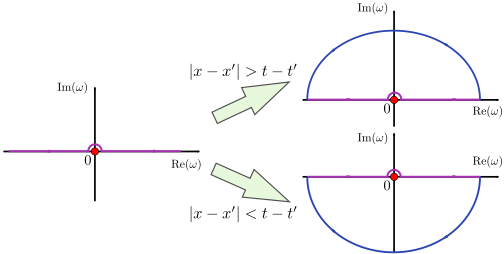
\includegraphics[width=0.75\textwidth]{causality_contour}
\end{figure}

The contour integral can be solved by either closing the contour in
the upper half-plane, or in the lower half-plane. If we close the
contour above, then the loop contour does not enclose the pole, and
hence $G(x,x';t-t') = 0$. According to Jordan's lemma, we must do this
if the exponent in the integrand obeys
\begin{equation}
  |x-x'| - (t-t') > 0  \quad \Rightarrow \quad |x-x'| > t-t'.
\end{equation}
This inequality is satisfied in two cases: either (i) $t < t'$ (in
which case the inequality is satisfied for all $x,x'$ because $|x-x'|$
is strictly non-negative), or (ii) $t > t'$ but the value of $t-t'$ is
smaller than $|x-x'|$. To understand the physical meaning of these two
cases, recall that $G(x,x';t-t')$ represents the field at position $x$
and time $t$ resulting from a pulse at the space-time point
$(x',t')$. Thus, case (i) corresponds to times occurring before the
pulse, and case (ii) corresponds to times occurring after the pulse
but positions which are too far away from the location of the pulse
for a wave to reach $x$ from $x'$.

By contrast, for $|x-x'| - (t-t') < 0$ we can use the residue theorem
to obtain $G(x,x';t-t') = -1/2$. From this description, it is clear
that the resulting time-domain Green's function is causal. Unlike the
harmonic oscillator case, causality for the wave equation imposes the
addition requirement that waves must be given enough time to propagate
between two specified points.

The time-domain wavefunction can therefore be written as
\begin{equation}
  \psi(x,t) = \int_{-\infty}^\infty dx' \int_{-\infty}^\infty dt'
  \left[-\frac{1}{2}\,\Theta(t-t' - |x-x'|)\right] f(x',t'),
\end{equation}
where $\Theta$ denotes the unit step function. In other words, the
wavefunction at each space-time point $(x,t)$ receives equal
contribution from the sources $f(x',t')$ at space-time points
$(x',t')$ which lie within the ``past light cone''.

\section{Looking ahead}

Green's functions are widely used to describe the emission of acoustic
and electromagnetic waves, and how they interact with various sorts of
media. This is a vast topic whose details are covered in advanced
courses in theoretical physics and electrical engineering. Here, we
give a brief sketch of some future directions of study.

So far, we have focused our attentions on the simplest case of an
infinite one-dimensional uniform medium. In most practical
applications, one is interested in three spatial dimensions, and in
non-uniform media. For such cases, the wave equation's
\hyperref[frequency-domain]{frequency-domain Green's function} can be
generalized to
\begin{equation}
  \left[\nabla^2 + n^2(\vec{r}) \, \left(\frac{\omega}{c}\right)^2\right]\, G(\vec{r},\vec{r}';\omega) = \delta^3(\vec{r}-\vec{r}'),  
\end{equation}
where $\nabla^2 = \partial^2/\partial x^2 + \partial^2/\partial y^2 +
\partial^2/\partial z^2$ is the three-dimensional Laplacian operator,
and $n(\vec{r})$ is the refractive index (see the discussion in
Chapter 5). On the right-hand side of this equation is the
three-dimensional delta function (see Section 9.5), which describes a
point source located at position $\vec{r}'$ in the three-dimensional
space.

When $n = 1$, the above equation is similar to the frequency-domain
Green's function equation \hyperref[outgoing]{that we studied in
  Section~\ref{outgoing}}, except that the problem is
three-dimensional rather than one-dimensional. Again assuming
\hyperref[outgoing]{outgoing boundary conditions
  (Section~\ref{outgoing})}, the solution for the Green's function in
three dimensions can be determined analytically. We will not cover the
solution method, but the result turns out to be
\begin{equation}
  G(\vec{r},\vec{r}';\omega) = -\frac{e^{i(\omega/c)|\vec{r}-\vec{r}'|}}{4\pi|\vec{r}-\vec{r}'|}.  
\end{equation}
Similar to the \hyperref[outgoing]{solution in one dimension}, this
depends on the distance from the source, $|\vec{r}-\vec{r}'|$, and
thus describes waves that are emitted isotropically from the source at
$\vec{r}'$. One difference is that the value of $G$ now decreases to
zero with distance, due to the $|\vec{r}-\vec{r}'|$ in the
denominator. This matches our everyday experience that the sound
emitted from a point source grows fainter with distance, and it
happens because the energy carried by the outgoing wave is spread out
over a larger area with increasing distance from the source. By
contrast, in one-dimensional space, the emitted waves do not spread as
they travel, and hence $G$ does not decrease with distance.

When $n(\vec{r})$ is not a constant but varies with position
$\vec{r}$, then the waves emitted by the source do not radiate
outwards in a simple way. The variations in the refractive index cause
the waves to scatter in complicated ways. In most situations, the
exact solution for the Green's function cannot be obtained
analytically, but must be computed using specialized numerical
methods. If the variations in $n(\vec{r})$ are sufficiently weak, one
can sometimes derive approximate expressions for the Green's function,
using a family of techniques known as \textbf{perturbation theory}.

For electromagnetic waves, there is another important complication:
electromagnetic fields are described by vectors (i.e., the electric
field vector and the magnetic field vector), not scalars.  The
propagation of electromagnetic waves is therefore described by a
vectorial wave equation, not the scalar wave equation that we have
assumed so far. Moreover, electromagnetic waves are not generated by
scalar sources, but by vector sources (electrical currents). The
corresponding Green's function is not a scalar quantity, but something
called a \textbf{dyadic Green's function}. This is a tensorial object
that describes the \emph{vector} waves emitted by a \emph{vector}
source.

Finally, even though we have dealt so far with classical (non-quantum)
waves, the Green's function concept is also crucial to the theory of
\emph{quantum} waves. \textbf{Quantum field theory} describes how
fields like the electromagnetic field behave according to the laws of
quantum mechanics. In this theory, the Green's functions no longer
have simple numerical values, but are quantum mechanical
\emph{operators}. Almost all problems in quantum field theory
essentially involve calculating a quantum mechanical Green's
function. Quantum field theory is widely used in the subjects of
condensed-matter physics and high-energy particle physics.

\section{Exercises}\label{exercises}

\begin{enumerate}
\item 
Find the time-domain Green's function of the critically-damped harmonic
oscillator, for which $\gamma = \omega_0$.

\item
Consider an overdamped harmonic oscillator ($\gamma > \omega_0$)
subjected to a \emph{random} driving force $f(t)$, which fluctuates
between random values, which can be either positive or negative, at each
time $t$. The random force satisfies
\begin{equation}
\left\langle f(t)\right\rangle = 0 \quad\mathrm{and}\;\;\;\left\langle f(t) f(t')\right\rangle = A \delta(t-t'),
\end{equation}
where $\left\langle\cdots\right\rangle$ denotes an average taken over
many realizations of the random force and $A$ is some constant which
characterizes the overall magnitude of the random force. Using the
causal Green's function, compute the ``correlation function''
$\left\langle x(t_1)\, x(t_2) \right\rangle$. Hence, show that for
small time displacements $\Delta t$, the motion obeys
\begin{equation}
\left\langle [x(t+\Delta t) - x(t)]^2 \right\rangle \propto D \Delta t.
\end{equation}
Compute the ``diffusion constant'' $D$. This result is called the
\textbf{fluctuation-dissipation theorem}, which relates the strength of
the fluctuations in a mechanical motion to the ``diffusiveness'' of its
motion.
\end{enumerate}

\end{document}
